%% Machine Learning with Applications — Elsevier
%% Versión en español simplificada (v2)
%%
%% Compilar:
%%   pdflatex main_es_v2
%%   bibtex   main_es_v2
%%   pdflatex main_es_v2
%%   pdflatex main_es_v2

\documentclass[preprint,12pt,authoryear]{elsarticle}

%% ── Paquetes ──────────────────────────────────────────────────────────────
\usepackage{amsmath,amssymb,amsfonts}
\usepackage{graphicx}
\usepackage{booktabs}
\usepackage{array}
\usepackage{multirow}
\usepackage[table,xcdraw]{xcolor}
\usepackage{hyperref}
\usepackage{cleveref}
\usepackage{lineno}
\usepackage{microtype}
\usepackage{siunitx}
\usepackage{bm}
\usepackage{caption}
\usepackage{subcaption}
\usepackage{enumitem}
\usepackage{algorithm}
\usepackage{algpseudocode}
\algrenewcommand\algorithmicwhile{\textbf{mientras}}
\algrenewcommand\algorithmicdo{\textbf{hacer}}
\algrenewcommand\algorithmicend{\textbf{fin}}
\algrenewcommand\algorithmicfor{\textbf{para}}
\algrenewcommand\algorithmicif{\textbf{si}}
\algrenewcommand\algorithmicthen{\textbf{entonces}}
\algrenewcommand\algorithmicelse{\textbf{si no}}
\algrenewcommand\algorithmicreturn{\textbf{retornar}}
\floatname{algorithm}{Algoritmo}
\usepackage[utf8]{inputenc}
\usepackage[T1]{fontenc}
\usepackage[spanish,es-nodecimaldot,es-noshorthands]{babel}

%% Numeración de líneas (requerida en revisión)
\linenumbers

\sisetup{separate-uncertainty=true, group-separator={.}, output-decimal-marker={,}}

\hypersetup{
    colorlinks=true,
    linkcolor=blue!70!black,
    citecolor=blue!60!black,
    urlcolor=blue!60!black
}

%% ── Macros ────────────────────────────────────────────────────────────────
\newcommand{\CR}[1]{CR_{2,\text{#1}}}
\newcommand{\RMSE}{\mathrm{RMSE_{VC}}}
\newcommand{\Rsq}{R^{2}_{\mathrm{VC}}}
\newcommand{\nd}{N_{\mathrm{d}}}
\newcommand{\np}{n_{\mathrm{p}}}
\newcommand{\etad}{\eta_{\mathrm{d}}}
\newcommand{\Mf}{M_{\!f}}
\newcommand{\ha}{h_a}
\newcommand{\KM}{\,\si{kN{\cdot}m}}

\journal{Machine Learning with Applications}

\begin{document}

\begin{frontmatter}

\title{Modelo Sustituto de Aprendizaje Automático para la Respuesta Sísmica
       No Lineal de Marcos de Acero con Amortiguadores de Fricción Rotacionales}

\author[uaq]{E.~Ponce}
\author[i2m]{H.~Yañez-Godoy\corref{cor1}}
\cortext[cor1]{Autor de correspondencia.}
\ead{humberto.yanez-godoy@u-bordeaux.fr}

\address[uaq]{Universidad Autónoma de Querétaro, Facultad de Ingeniería,
              Cerro de las Campanas s/n, Querétaro, México}
\address[i2m]{Arts et Metiers Institute of Technology, University of Bordeaux,
              Centre National de la Recherche Scientifique (CNRS),
              Bordeaux INP, I2M, UMR 5295, 33400 Talence, France}

%%─── Resumen ───────────────────────────────────────────────────────────────
\begin{abstract}
Este trabajo presenta un modelo sustituto de aprendizaje automático (ML) para
optimizar amortiguadores de fricción rotacionales (AFR) en marcos
de acero resistentes a momento (MARM). Se generaron 1\,000 marcos tipo cortante
(3--20~pisos, período fundamental $T_1 \in [0{,}3,\,3{,}0]$\,s) mediante
Muestreo por Hipercubo Latino (MHL). Para cada marco se evaluaron 50
configuraciones de AFR bajo 8 registros sísmicos reales, produciendo
$\approx$434\,000 simulaciones no lineales resueltas con el método de Dinámica
No Suave (DNS). El desempeño se mide con el índice $CR_2$, el cual combina 
desplazamiento máximo, la aceleración máxima y el cortante basal,
normalizados respecto a la estructura sin amortiguadores. Se calculan tres
estadísticos por configuración: mediana (típico), P10 (favorable) y P90
(conservador). Cuatro modelos de regresión fueron entrenados con validación
cruzada GroupKFold. XGBoost obtuvo el mejor resultado: $\Rsq = 0{,}92$,
$0{,}93$ y $0{,}84$ para $\CR{med}$, $\CR{P10}$ y $\CR{P90}$.
La densidad de cobertura $\etad = \nd/\np$ es la variable de diseño dominante
($r=-0{,}73$ con $CR_2$). El 80\,\% de la mejora máxima se alcanza con
$\etad \approx 0{,}85$ en marcos de mediana y gran altura (6--20~pisos),
estableciendo un umbral práctico de rendimiento decreciente.
\end{abstract}

\begin{keyword}
Rotational Friction Dampers \sep Machine Learning \sep Seismic Optimization \sep
Non-Smooth Dynamics \sep Steel Moment Frames \sep Surrogate Model \sep
Diminishing Returns
\end{keyword}

\end{frontmatter}

%%═══════════════════════════════════════════════════════════════════════════
\section{Introducción}
\label{sec:intro}
%%═══════════════════════════════════════════════════════════════════════════

Los amortiguadores de fricción rotacionales (AFR) son dispositivos pasivos que
mejoran el comportamiento sísmico de marcos de acero disipando energía por
fricción \citep{pall_friction_1980, pall_response_1982, jaisee_state---art_2021}.
\citet{Mualla2002} los propuso e investigó experimentalmente, mostrando que
disipan hasta el 89\,\% de la energía de entrada en ensayos a escala. Para un
caso optimizado con el registro El~Centro NS, reportó reducciones del 89\,\% en
desplazamiento lateral y del 41\,\% en cortante basal respecto al sistema sin
amortiguamiento.

A diferencia de los marcos convencionales, donde la energía sísmica se disipa
dañando los miembros estructurales, los AFR transfieren esa energía a un
mecanismo friccional no estructural. Así se protegen los elementos principales
y se logra un comportamiento sísmico más predecible
\citep{de_domenico_editorial_2020}.

Sin embargo, modelar la fricción seca es difícil porque el comportamiento cambia
de forma abrupta entre deslizamiento y reposo. Algunos estudios usan modelos
simplificados (bilineal o amortiguamiento equivalente) que no capturan bien estas
transiciones \citep{lee_seismic_2025, Jarrahi2020jbe}. \citet{Namorado2024}
propuso formular los AFR con el método de Dinámica No Suave (DNS), que trata la
fricción de Coulomb como una inclusión diferencial-algebraica. Esto permite
representar directamente los estados de adherencia y deslizamiento sin
aproximaciones.

Varios trabajos han optimizado amortiguadores con algoritmos metaheurísticos
\citep{moreschi_design_2003, moghaddam_optimal_2022, miguel_simultaneous_2016,
ontiveros-perez_reliability-based_2019}. \citet{Jarrahi2020jbe} y
\citet{Jarrahi2020sdee} optimizaron AFR con criterios energéticos, encontrando
que agregar más dispositivos deja de ser útil alrededor del 60\,\% de cobertura.
Pero estos estudios usan un solo registro sísmico y una estructura específica,
lo que limita aplicar sus resultados a edificios de diferente altura.

El aprendizaje automático (ML) permite construir modelos que predicen el
desempeño sísmico con un costo computacional mucho menor que el análisis no
lineal \citep{Kazemi2022}. El espacio de diseño de AFR ---combinaciones de
ubicación, número y capacidad de dispositivos--- es de alta dimensión y
presenta relaciones no lineales con la respuesta sísmica que los enfoques
analíticos no capturan eficientemente, lo que hace del ML una herramienta
apropiada para este problema. Un estudio previo del grupo de investigación
\citep{Ponce2026} aplicó el método DNS a un marco de 10~pisos bajo cinco
registros sísmicos, identificando un punto de saturación en 7~amortiguadores y
momentos friccionales óptimos de 350--450\KM, lo que motivó extender el análisis
a un espacio de diseño de mayor amplitud.

Las contribuciones de este artículo son: (i)~una base de datos de 1\,000
estructuras $\times$ 50 configuraciones $\times$ 8 registros sísmicos, generada
con DNS; (ii)~un umbral práctico de rendimiento decreciente
($\etad \approx 0{,}85$), que extiende el resultado del 60\,\% de
\citet{Jarrahi2020sdee} al incluir desplazamientos y aceleraciones; y
(iii)~un modelo sustituto ML con validación cruzada para explorar el espacio de
diseño bajo variabilidad sísmica multi-registro.

El artículo se organiza así: la \cref{sec:theory} presenta el marco teórico;
la \cref{sec:method} describe la metodología; la \cref{sec:results} muestra
los resultados; la \cref{sec:discussion} discute las implicaciones; y la
\cref{sec:conclusions} resume las conclusiones.

%%═══════════════════════════════════════════════════════════════════════════
\section{Marco Teórico}
\label{sec:theory}
%%═══════════════════════════════════════════════════════════════════════════

\subsection{Amortiguador de Fricción Rotacional}
\label{sec:theory:afr}

Los AFR disipan energía mediante el deslizamiento entre superficies en contacto.
El dispositivo de \citet{Mualla2002} tiene una placa central, dos placas
laterales, discos de material friccional y un perno pretensado. La compresión
del perno activa la fricción y genera ciclos histéreticos estables cuya área
es la energía disipada. La \cref{fig:rfd} muestra los componentes.

\begin{figure}[htbp]
    \centering
    \begin{subfigure}[b]{0.48\textwidth}
        \centering
        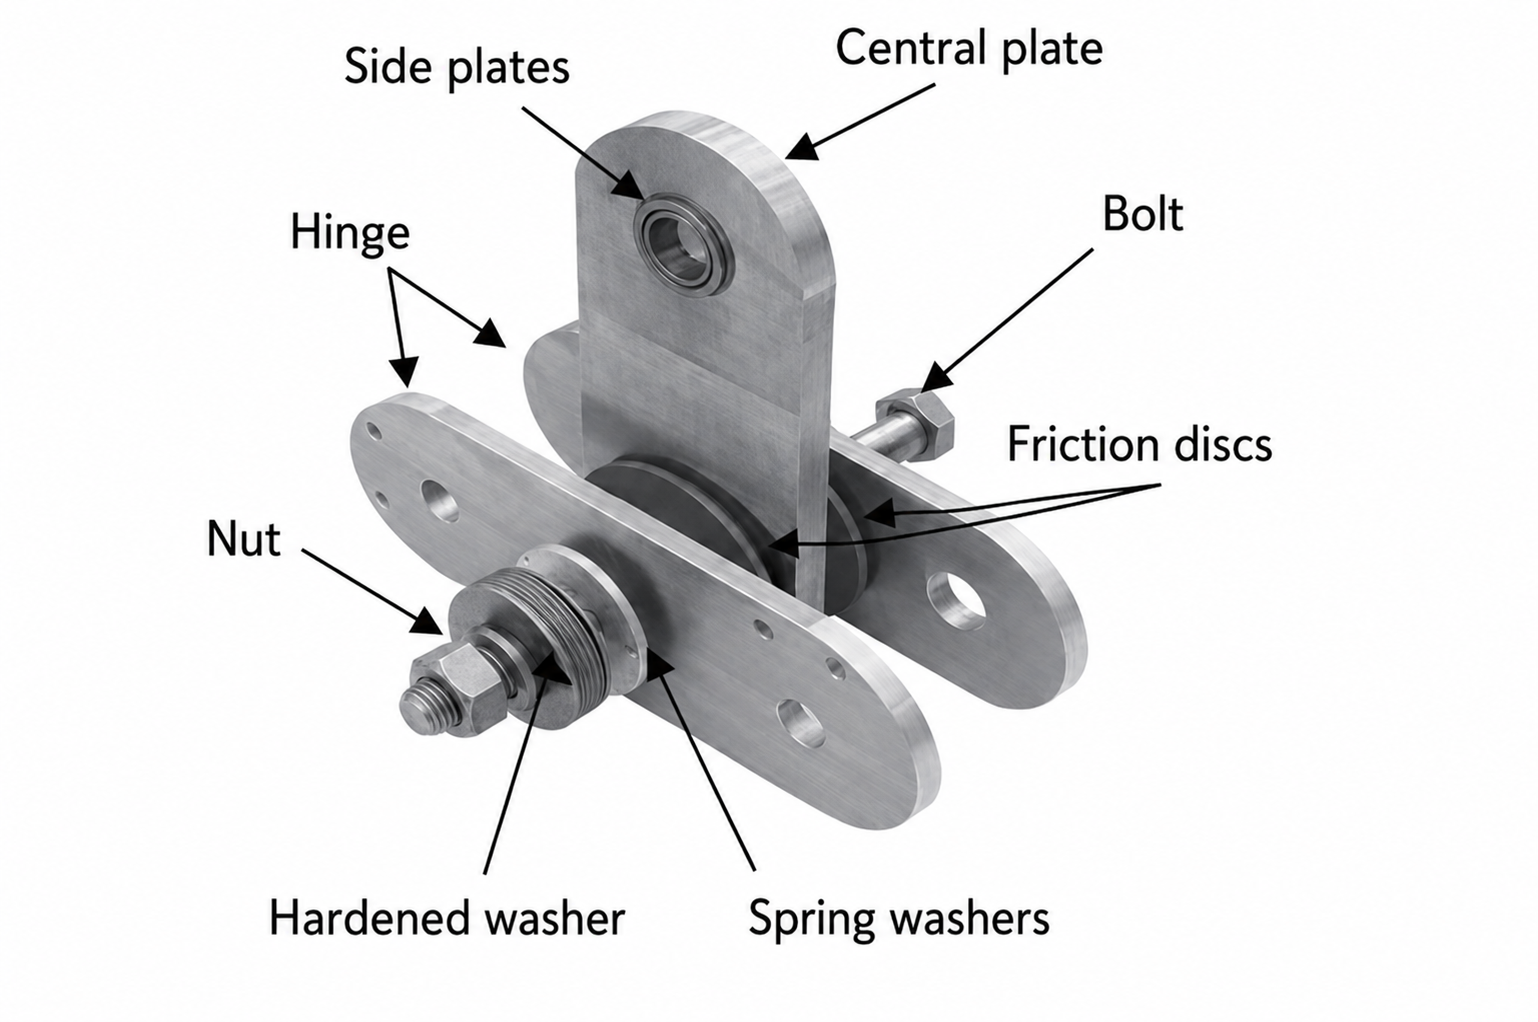
\includegraphics[width=\textwidth]{rfd_componentes.png}
        \caption{Componentes del AFR: placa central, placas laterales,
                 discos de fricción, perno pretensado y arandelas.}
        \label{fig:rfd_componentes}
    \end{subfigure}
    \hfill
    \begin{subfigure}[b]{0.48\textwidth}
        \centering
        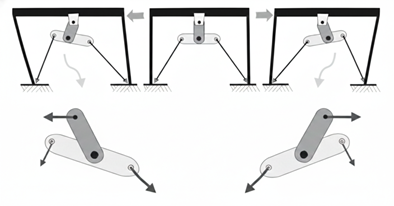
\includegraphics[width=\textwidth]{rfd_mecanismo.png}
        \caption{Mecanismo de actuación: el desplazamiento lateral del
                 marco induce la rotación en el dispositivo, disipando
                 energía por fricción.}
        \label{fig:rfd_mecanismo}
    \end{subfigure}
    \caption{Amortiguador de Fricción Rotacional (AFR). Izquierda: configuración
             física del dispositivo \citep{Mualla2002}. Derecha: activación bajo
             excitación sísmica lateral.}
    \label{fig:rfd}
\end{figure}

La placa central se conecta a la viga y las laterales al arriostramiento. Cuando
el marco se mueve lateralmente por un sismo, el movimiento relativo entre pisos
hace rotar el dispositivo, generando fricción. Así, la energía que dañaría el
marco se transfiere al AFR \citep{kim_use_2011}.

La capacidad se expresa como momento friccional máximo $\Mf$. La fuerza lateral
equivalente que transmite es:
\begin{equation}
    F_{\mathrm{afr}} = \frac{\Mf}{\ha},
    \label{eq:Fafr}
\end{equation}
donde $\ha$ es el brazo de palanca del arriostramiento. \citet{Mualla2002}
verificaron que el comportamiento es independiente de la frecuencia en 2--7\,Hz,
lo que justifica usar la ley de Coulomb.

\subsection{Análisis Dinámico con Dinámica No Suave}
\label{sec:theory:dns}

La fricción de Coulomb cambia de forma abrupta entre deslizamiento y reposo,
lo que los integradores convencionales manejan mal \citep{chopra_dynamics_2015}.
Para resolver esto sin linealizar, se usa el método DNS de \citet{Namorado2024},
que trabaja con velocidades e impulsos en lugar de aceleraciones y fuerzas
instantáneas.

\subsubsection*{Ley de fricción}

Para un AFR entre los pisos $i$ e $i+1$, el momento resistente sigue la ley de
Coulomb:
\begin{equation}
    M_{\mathrm{afr},i} \in -\Mf \cdot \operatorname{Sign}\!\left(\dot{\varphi}_i\right),
    \label{eq:coulomb}
\end{equation}
con el signo extendido:
\begin{equation}
    \operatorname{Sign}(v) =
    \begin{cases}
        \{+1\}    & \text{si } v > 0, \\
        [-1,\,+1] & \text{si } v = 0, \\
        \{-1\}    & \text{si } v < 0.
    \end{cases}
    \label{eq:sign}
\end{equation}
Si el dispositivo desliza, el momento es $\pm\Mf$. En reposo, puede tomar
cualquier valor en $[-\Mf,\,+\Mf]$ según el equilibrio.

\subsubsection*{Ecuación de movimiento}

El sistema de $\np$ pisos con $n_a$ amortiguadores sigue la inclusión diferencial
\citep{Namorado2024}:
\begin{equation}
    \bm{M}\,\ddot{\bm{u}} + \bm{C}\,\dot{\bm{u}} + \bm{K}\,\bm{u}
    \in -\bm{M}\,\bm{r}\,\ddot{x}_g(t) + \bm{H}\,\bm{Q}_f(t),
    \label{eq:eom}
\end{equation}
donde $\bm{M}$, $\bm{C}$ y $\bm{K}$ son las matrices de masa, amortiguamiento
y rigidez; $\bm{u}$ es el desplazamiento relativo al suelo; y $\bm{H}$ indica
en qué pisos está cada amortiguador. En la versión discreta, la fuerza
multivaluada se reemplaza por impulsos $\bm{\lambda}_{k+1}$ calculados en cada
paso mediante un Problema de Complementariedad Lineal (LCP, ec.~\ref{eq:lcp}):
\begin{equation}
    \bm{M}\,\ddot{\bm{u}} + \bm{C}\,\dot{\bm{u}} + \bm{K}\,\bm{u}
    = -\bm{M}\,\bm{r}\,\ddot{x}_g(t) + \bm{H}\,\bm{\lambda}_{k+1}/\Delta t.
    \label{eq:eom_disc}
\end{equation}

\subsubsection*{Procedimiento NSD-LCP-PSOR}

El algoritmo avanza de $k$ a $k+1$ en tres pasos (Algoritmo~\ref{alg:nsd-lcp-psor}).

\textbf{Predictor.} Se calcula la velocidad del sistema sin fuerza de fricción,
usando la matriz de masa modificada:
\begin{equation}
    \hat{\bm{M}} = \bm{M}
                  + \theta\Delta t\,\bm{C}
                  + (\theta\Delta t)^{2}\bm{K},
    \label{eq:Mhat}
\end{equation}
lo que da:
\begin{equation}
    \dot{\bm{u}}^{\mathrm{libre}} = \hat{\bm{M}}^{-1}
    \!\left[
        \bm{A}\,\dot{\bm{u}}_k
        - \Delta t\,\bm{K}\bm{u}_k
        - \theta\Delta t\,\bm{M}\!\left(\ddot{x}_{g,k+1}+\ddot{x}_{g,k}\right)\bm{r}
    \right],
    \label{eq:vfree}
\end{equation}
con $\bm{A} = \bm{M} - \theta\Delta t\,\bm{C} - (\theta\Delta t)^{2}\bm{K}$.

\textbf{Corrector.} Se calculan los impulsos $\bm{\lambda}_{k+1}$ que satisfacen
la ley de Coulomb resolviendo el LCP:
\begin{equation}
    \bm{W}\bm{\lambda} + \bm{q} = \bm{0},
    \quad |\lambda_r| \leq \frac{\Mf\,\Delta t}{\ha},
    \quad r = 1,\ldots,n_a,
    \label{eq:lcp}
\end{equation}
donde $W_{rs} = [\bm{H}^{\top}\hat{\bm{M}}^{-1}\bm{H}]_{rs}\Delta t$ y
$q_r$ es la velocidad relativa libre en cada dispositivo. El LCP se resuelve
con PSOR (\textit{Projected Successive Over-Relaxation}): se actualiza cada
impulso en secuencia y se proyecta sobre el intervalo admisible.

\textbf{Actualización de estado.}
\begin{align}
    \dot{\bm{u}}_{k+1} &= \dot{\bm{u}}^{\mathrm{libre}}
        + \Delta t\,\hat{\bm{M}}^{-1}\bm{H}\bm{\lambda}_{k+1}, \label{eq:vupdate}\\
    \bm{u}_{k+1} &= \bm{u}_k
        + \Delta t\!\left[(1-\theta)\,\dot{\bm{u}}_k
                         + \theta\,\dot{\bm{u}}_{k+1}\right]. \label{eq:uupdate}
\end{align}
El impulso del paso $k$ sirve como punto de partida en $k+1$, reduciendo
las iteraciones necesarias.

\begin{algorithm}[t]
\caption{NSD-LCP-PSOR aplicado a marcos MDOF con AFR}
\label{alg:nsd-lcp-psor}
\begin{algorithmic}[1]
\Require $\bm{M},\bm{C},\bm{K}$; $\bm{H}$, $\bm{F}^{\lim}$;
         $\{\ddot{x}_{g,k}\}_{k=0}^{n}$; $\Delta t$, $\theta$
\Ensure  $\{\bm{u}_k,\dot{\bm{u}}_k\}_{k=0}^{n}$
\vspace{2pt}
\State \textit{// Pre-cómputo (una sola vez)}
\State $\hat{\bm{M}} \leftarrow \bm{M} + \theta\Delta t\,\bm{C} + (\theta\Delta t)^{2}\bm{K}$
\State $\bm{A} \leftarrow \bm{M} - \theta\Delta t\,\bm{C} - (\theta\Delta t)^{2}\bm{K}$
\State $\bm{W} \leftarrow \left(\bm{H}^{\top}\hat{\bm{M}}^{-1}\bm{H}\right)\Delta t$
\State $\bm{u}_0 \leftarrow \bm{0}$;\quad $\dot{\bm{u}}_0 \leftarrow \bm{0}$;\quad
       $\bm{\lambda}_0 \leftarrow \bm{0}$
\vspace{2pt}
\For{$k = 0, 1, \ldots, n-1$}
    \State \textit{// Paso 1 — velocidad libre}
    \State $\bm{b}_k \leftarrow \bm{A}\,\dot{\bm{u}}_k
            - \Delta t\,\bm{K}\bm{u}_k
            - \theta\Delta t\,\bm{M}\!\left(\ddot{x}_{g,k+1}+\ddot{x}_{g,k}\right)\bm{r}$
    \State $\dot{\bm{u}}^{\mathrm{lib}} \leftarrow \hat{\bm{M}}^{-1}\bm{b}_k$
    \State \textit{// Paso 2 — velocidades relativas libres}
    \State $q_r \leftarrow \dot{u}^{\mathrm{lib}}_{f_r} - \dot{u}^{\mathrm{lib}}_{f_r-1}$
           \quad para $r = 1,\ldots,n_a$
    \State \textit{// Paso 3 — PSOR (corrector)}
    \State $\bm{\lambda}^{(0)} \leftarrow \bm{\lambda}_k$
    \While{$\|\bm{\lambda}^{(i+1)} - \bm{\lambda}^{(i)}\|_\infty > \varepsilon$}
        \For{$r = 1,\ldots,n_a$}
            \State $\tilde{\lambda}_r \leftarrow
                   -\!\left(q_r + \sum_{s \neq r} W_{rs}\lambda_s^{(i)}\right)\!\big/W_{rr}$
            \State $\lambda_r^{(i+1)} \leftarrow
                   \max\!\left(-F^{\lim}_r,\;\min\!\left(F^{\lim}_r,\;\tilde{\lambda}_r\right)\right)$
        \EndFor
    \EndWhile
    \State $\bm{\lambda}_{k+1} \leftarrow \bm{\lambda}^{(*)}$
           \quad\textit{($F^{\lim}_r = \Mf\Delta t/\ha$)}
    \State \textit{// Paso 4 — actualización}
    \State $\dot{\bm{u}}_{k+1} \leftarrow
           \dot{\bm{u}}^{\mathrm{lib}} +
           \Delta t\,\hat{\bm{M}}^{-1}\bm{H}\bm{\lambda}_{k+1}$
    \State $\bm{u}_{k+1} \leftarrow \bm{u}_k +
           \Delta t\!\left[(1-\theta)\,\dot{\bm{u}}_k +
                           \theta\,\dot{\bm{u}}_{k+1}\right]$
\EndFor
\end{algorithmic}
\end{algorithm}

El paso de tiempo $\Delta t = 0{,}01$\,s coincide con el intervalo de muestreo
de los registros sísmicos, evitando interpolación. Para las estructuras más
rígidas ($T_1 = 0{,}3$\,s) esto da 30 puntos por período, cumpliendo el criterio
$\Delta t / T_1 \leq 0{,}10$ \citep{chopra_dynamics_2015}. La fuerza friccional
en el piso $i$ es:
\begin{equation}
    f_{\mathrm{afr},i} = \frac{\lambda_i}{\ha\,\Delta t}.
    \label{eq:ffrict}
\end{equation}

\subsubsection*{Adaptación del DNS para simulación masiva MDOF}

El método de \citet{Namorado2024} fue validado para marcos de uno a cinco pisos.
La implementación NSD-LCP-PSOR desarrollada en este trabajo fue previamente
verificada en \citet{Ponce2026} para un marco cortante de 10~pisos sometido a
cinco registros sísmicos reales bajo un marco probabilístico Monte Carlo,
comprobando ciclos histéreticos y respuestas de desplazamiento consistentes con
la literatura. Para aplicarlo a marcos de hasta veinte pisos se realizaron tres
ajustes adicionales.

\textbf{LCP conjunto.} Los impulsos de todos los amortiguadores se resuelven al
mismo tiempo con la matriz $\bm{W}$, que recoge cómo interactúan los dispositivos
a través de la estructura.

\textbf{Sin parámetro de ajuste.} El algoritmo original tiene un parámetro
$\alpha$ que hay que elegir por caso. Al formular el problema como LCP ese
parámetro desaparece, lo que facilita aplicarlo a miles de configuraciones.

\textbf{Reutilización del impulso.} El impulso del paso anterior sirve de punto
de partida, reduciendo las iteraciones porque la respuesta cambia poco entre
pasos.

\subsection{Métrica de Desempeño Sísmico}
\label{sec:theory:metrica}

El desempeño de cada configuración se mide con razones normalizadas respecto a
la estructura sin amortiguadores \citep{Namorado2024, Jarrahi2020jbe, Mualla2002}:
\begin{equation}
    R_1 = \frac{u_{\max}^{(\mathrm{c})}}{u_{\max}^{(0)}}, \quad
    R_2 = \frac{\ddot{u}_{\max}^{(\mathrm{c})}}{\ddot{u}_{\max}^{(0)}}, \quad
    R_3 = \frac{V_{\max}^{(\mathrm{c})}}{V_{\max}^{(0)}},
    \label{eq:R_individual}
\end{equation}
donde (c) es la estructura con amortiguadores y (0) sin ellos. Con estas razones
se construyen dos índices:
\begin{equation}
    CR_1 = \sqrt{R_1^2 + R_2^2}, \qquad
    CR_2 = \sqrt{R_1^2 + R_2^2 + R_3^2}.
    \label{eq:CR}
\end{equation}
Sin amortiguadores, $CR_2 = \sqrt{3}$; valores menores indican mejora. Dado
que $CR_2$ depende del registro, se resume en tres estadísticos
\citep{Kazemi2022}:
\begin{align}
    \CR{P10} &= Q_{0{,}10}\!\left(\{CR_2^{(k)}\}_{k=1}^{N_r}\right), \quad
    \CR{med}  = Q_{0{,}50}\!\left(\{CR_2^{(k)}\}_{k=1}^{N_r}\right), \notag\\
    \CR{P90} &= Q_{0{,}90}\!\left(\{CR_2^{(k)}\}_{k=1}^{N_r}\right).
    \label{eq:CR2stats}
\end{align}
$\CR{P10}$ representa una condición favorable, $\CR{med}$ el comportamiento
típico y $\CR{P90}$ una condición severa.

\subsection{Aprendizaje Automático para Optimización Estructural}
\label{sec:theory:ml}

Se entrena una función de regresión $\hat{y} = f(\bm{x};\,\bm{\theta})$ que
mapea variables de diseño $\bm{x}$ a un estadístico de $CR_2$. El entrenamiento
minimiza el error cuadrático medio:
\begin{equation}
    \mathcal{L}(\bm{\theta}) = \frac{1}{N}\sum_{i=1}^{N}
    \bigl(y_i - f(\bm{x}_i;\,\bm{\theta})\bigr)^2.
    \label{eq:mse}
\end{equation}
Se comparan cuatro algoritmos: Regresión Lineal y Ridge como referencias;
Random Forest \citep{Breiman2001}, que promedia múltiples árboles; y XGBoost
\citep{Chen2016}, que los construye secuencialmente corrigiendo errores. La
generalización se evalúa con GroupKFold de cinco particiones \citep{Kazemi2022},
agrupando por identificador de estructura. Las métricas son:
\begin{equation}
    \RMSE = \sqrt{\frac{1}{|V|}\sum_{i \in V}\bigl(y_i - \hat{y}_i\bigr)^2},
    \qquad
    \Rsq  = 1 - \frac{\sum_{i \in V}(y_i - \hat{y}_i)^2}
                      {\sum_{i \in V}(y_i - \bar{y})^2},
    \label{eq:metrics}
\end{equation}
donde $\hat{y}_i$ son las predicciones fuera de muestra (\textit{out-of-fold}).

%%═══════════════════════════════════════════════════════════════════════════
\section{Metodología}
\label{sec:method}
%%═══════════════════════════════════════════════════════════════════════════

\subsection{Diseño de Experimentos}
\label{sec:method:doe}

Se usó MHL \citep{McKay1979} para generar 1\,000 marcos tipo cortante. Cada uno
queda definido por: número de pisos $\np \in \{3, 5, 7, 10, 12, 15, 18, 20\}$;
período $T_1 \in [0{,}3,\,3{,}0]$\,s; masa por nivel $\bar{m} \in [150,\,350]$\,t;
perfil de masa (uniforme, lineal ascendente, descendente o concentrada en parte
alta); y perfil de rigidez (uniforme, lineal ascendente, descendente o piso
suave en la base). La rigidez se calibró analíticamente para cumplir el $T_1$
objetivo mediante $(\bm{K} - \omega_1^2\,\bm{M})\,\bm{\phi}_1 = \bm{0}$.

Para cada estructura se generaron $\approx 50$ configuraciones de AFR: 40 con
MHL sobre el espacio binario de ubicación y $\Mf \in [25,\,500]$\KM, y 10
orientadas a coberturas específicas. La presencia de un AFR en el piso $i$ se
indica con $b_i = 1$, dando $\nd = \|\bm{b}\|_0$ y $\etad = \nd/\np$. El plan
total es 433\,984 simulaciones.

\subsection{Modelos Estructurales y Análisis Dinámico}
\label{sec:method:modelo}

Cada estructura es un marco cortante lineal con masas concentradas por nivel y
amortiguamiento de Rayleigh con $\zeta = 3\,\text{\%}$, calibrado a los modos
1 y 3 \citep{chopra_dynamics_2015}. Los ocho acelerogramas son: El~Centro~1940,
Jamiltepec~2018, Kobe~1995, Loma Prieta~1989, Niltepec~2017, Northridge~1994,
Trinidad~1983 y Zacatula~1997. La integración usa el esquema DNS con
$\Delta t = 0{,}01$\,s y brazo de palanca $\ha = 0{,}40$\,m
\citep{Mualla2002, Jarrahi2020jbe}.

\subsection{Ingeniería de Características}
\label{sec:method:features}

Las cuatro variables primarias de diseño no capturan información espacial de la
configuración. Se añaden cinco características derivadas que compactan esta
información de forma explícita. El vector completo tiene 29 predictores:

\begin{enumerate}[label=\textit{\roman*})]
    \item \textbf{Variables de diseño primarias} (4):
          $\np$, $T_1$, $\Mf$ y $\nd$.

    \item \textbf{Características derivadas} (5):
    \begin{itemize}
        \item $\etad = \nd/\np$: densidad de cobertura, variable dominante;
        \item $\bar{p} = \tfrac{1}{\nd}\sum_{i:\,b_i=1} i$: posición promedio;
        \item $\tilde{p} = \bar{p}/\np$: posición promedio normalizada;
        \item $\sigma_p = \mathrm{std}\!\left(\{i:b_i=1\}\right)/\np$:
              dispersión vertical normalizada;
        \item $\tilde{E} = E_{\mathrm{total}}/(\np\times10^6)$: energía
              disipada normalizada por piso.
    \end{itemize}

    \item \textbf{Indicadores binarios de ubicación} (20):
          $b_1,\ldots,b_{20}$, donde $b_i=1$ si el piso $i$ tiene un AFR;
          marcos con menos de 20 pisos se completan con ceros.
\end{enumerate}

\subsection{Entrenamiento y Validación}
\label{sec:method:entrenamiento}

Los tres objetivos se predicen de forma independiente. Los hiperparámetros son
estándar: Random Forest usa $n=100$ árboles y profundidad máxima 15; XGBoost
usa $n=100$ estimadores, profundidad máxima 6 y tasa de aprendizaje $\eta=0{,}1$.
La importancia de características es el decremento medio de impureza de XGBoost.

%%═══════════════════════════════════════════════════════════════════════════
\section{Resultados}
\label{sec:results}
%%═══════════════════════════════════════════════════════════════════════════

\subsection{Desempeño Predictivo de los Modelos ML}
\label{sec:results:desempenio}

La \cref{tab:desempenio} resume los resultados. Los modelos de ensemble reducen
el $\RMSE$ en un 49\,\% respecto a los lineales para $\CR{med}$ y un 40\,\% para
$\CR{P10}$. XGBoost tiene el menor error en $\CR{med}$ y $\CR{P10}$; Random
Forest tiene una ligera ventaja en $\CR{P90}$ (\cref{fig:comparacion_modelos}).

\begin{table}[h!]
\centering
\caption{RMSE y $R^2$ con validación cruzada por modelo y variable objetivo.
         GroupKFold de cinco particiones, agrupadas por identificador de
         estructura.}
\label{tab:desempenio}
\small
\setlength{\tabcolsep}{4pt}
\begin{tabular}{lcccccc}
\toprule
& \multicolumn{2}{c}{$\CR{med}$}
& \multicolumn{2}{c}{$\CR{P10}$}
& \multicolumn{2}{c}{$\CR{P90}$} \\
\cmidrule(lr){2-3}\cmidrule(lr){4-5}\cmidrule(lr){6-7}
Modelo & $\RMSE$ & $\Rsq$ & $\RMSE$ & $\Rsq$ & $\RMSE$ & $\Rsq$ \\
\midrule
Regresión Lineal & 0{,}1274 & 0{,}695 & 0{,}1267 & 0{,}812 & 0{,}1838 & 0{,}435 \\
Ridge            & 0{,}1274 & 0{,}695 & 0{,}1268 & 0{,}812 & 0{,}1838 & 0{,}435 \\
Random Forest    & 0{,}0681 & 0{,}913 & 0{,}0785 & 0{,}928 & 0{,}0981 & \textbf{0{,}839} \\
XGBoost          & \textbf{0{,}0652} & \textbf{0{,}920} & \textbf{0{,}0755} & \textbf{0{,}933} & 0{,}0984 & 0{,}838 \\
\bottomrule
\end{tabular}
\end{table}

\begin{figure}[htbp]
\centering
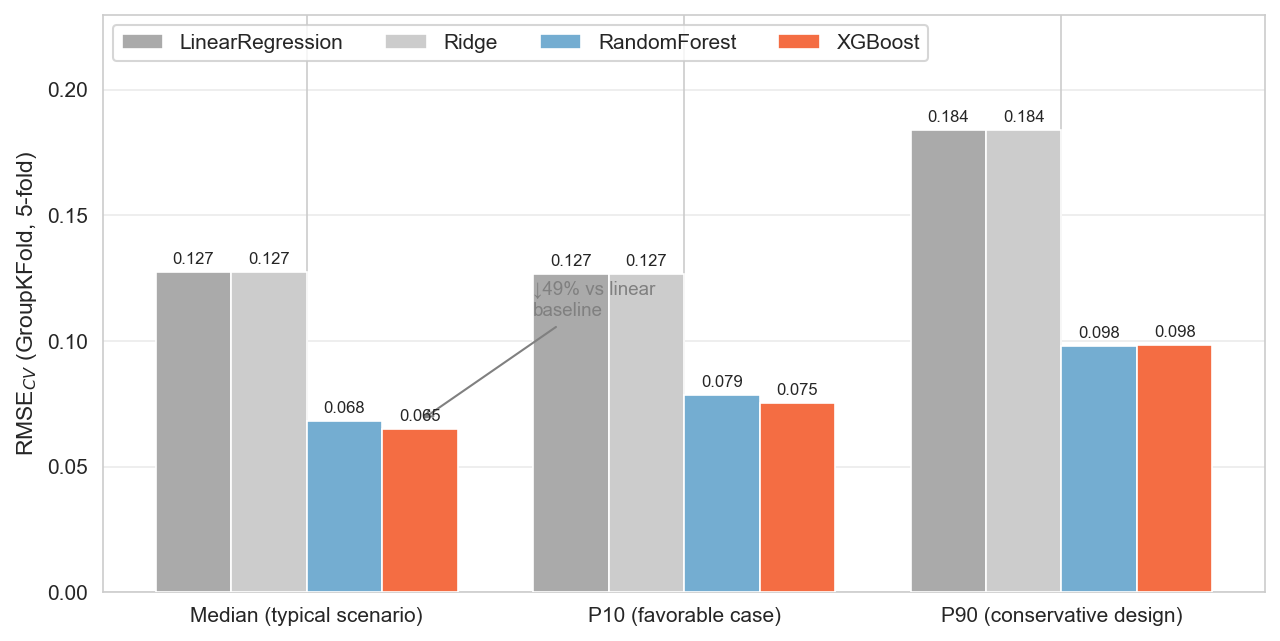
\includegraphics[width=0.85\linewidth]{figs/F1_model_comparison_rmse.png}
\caption{Comparación del $\RMSE$ con validación cruzada entre modelos y variables
objetivo. Los modelos de ensemble alcanzan aproximadamente la mitad del error de
los baselines lineales.}
\label{fig:comparacion_modelos}
\end{figure}

Para $\CR{P10}$ los modelos lineales alcanzan $\Rsq = 0{,}81$: en escenarios
favorables la relación es predominantemente lineal. El $\Rsq = 0{,}44$ para
$\CR{P90}$ bajo modelos lineales confirma que el escenario conservador tiene
interacciones no lineales que solo los ensemble capturan.

La \cref{fig:pred_vs_actual} muestra la dispersión OOF de XGBoost. Las
predicciones siguen la línea de identidad sin sesgo. Los residuales aumentan
para $CR_2 > 1{,}8$, zona de marcos bajos ($\np \leq 5$), donde la respuesta
es más sensible a variaciones pequeñas en los parámetros.

\begin{figure}[htbp]
\centering
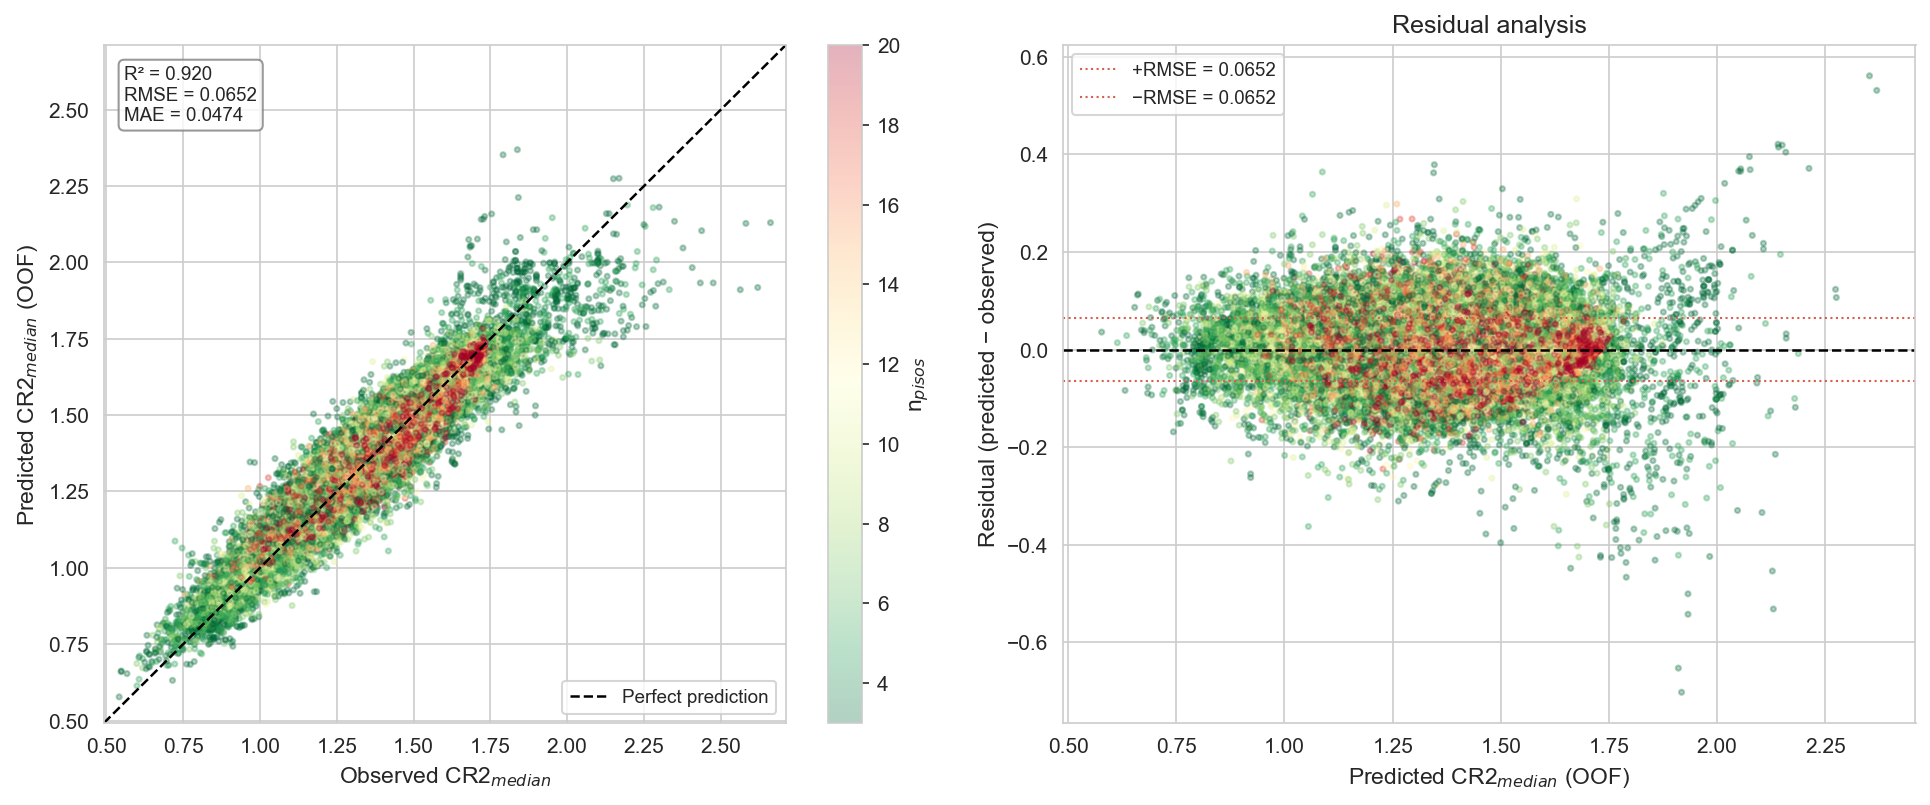
\includegraphics[width=\linewidth]{figs/F2_predicted_vs_actual_oof.png}
\caption{XGBoost OOF para $\CR{med}$. \textit{Izquierda}: predicción vs.\
valor observado; color: $\np$. \textit{Derecha}: residuales vs.\ predicho;
bandas: $\pm\RMSE$. $\Rsq = 0{,}92$, $\RMSE = 0{,}065$.}
\label{fig:pred_vs_actual}
\end{figure}

\begin{figure}[htbp]
\centering
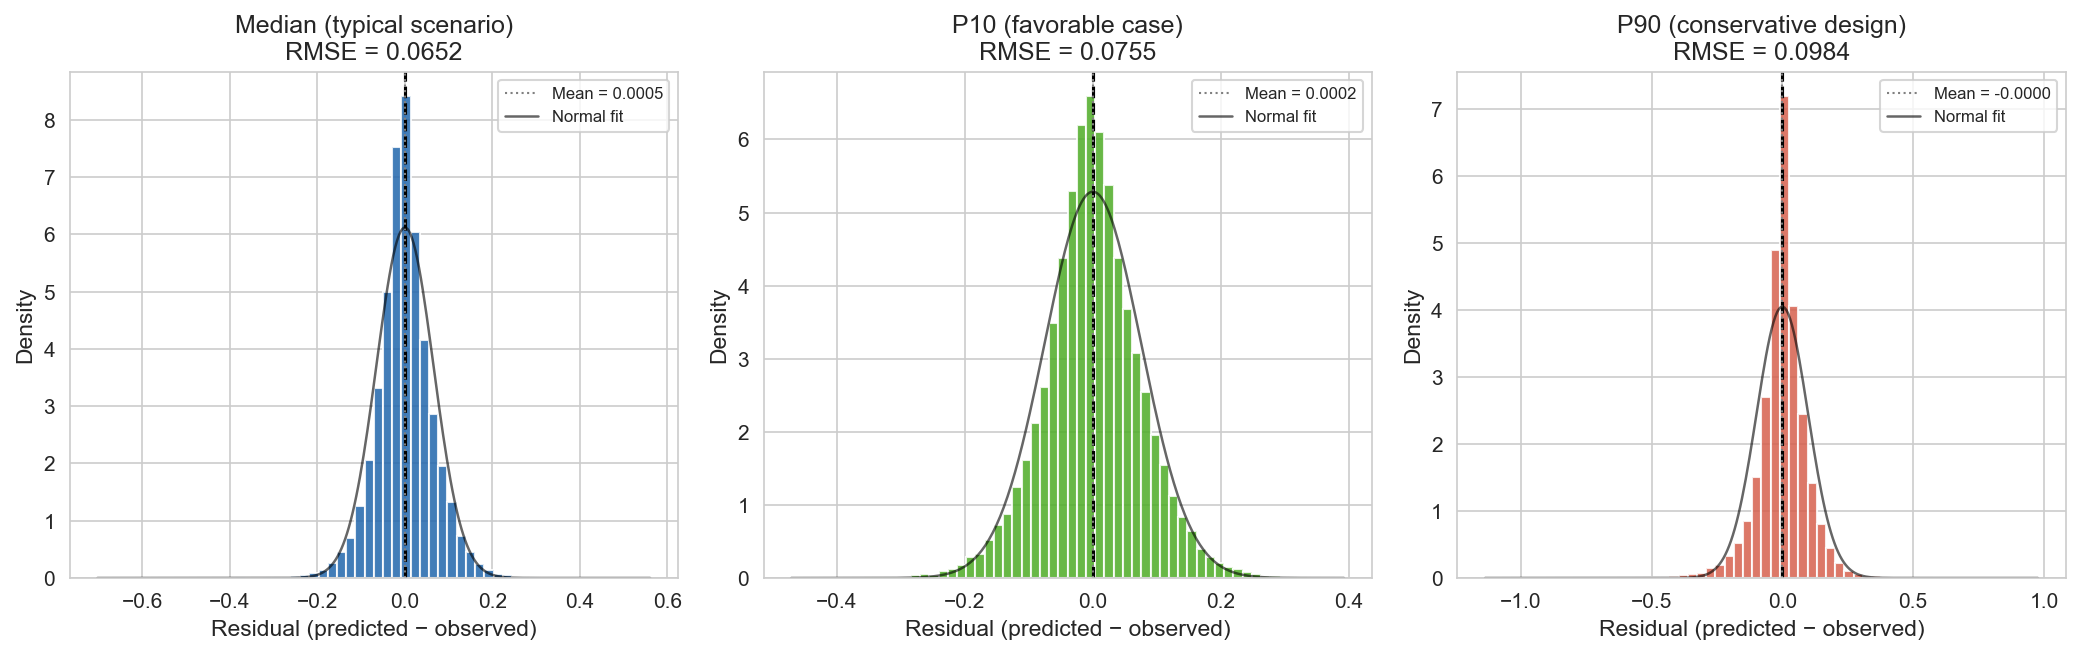
\includegraphics[width=\linewidth]{figs/F3_residual_distributions.png}
\caption{Distribuciones de residuales (OOF, XGBoost) para los tres objetivos
de $CR_2$. Línea punteada: media cero; curva sólida: ajuste normal.}
\label{fig:residuales}
\end{figure}

\subsection{Jerarquía de Variables e Importancia de Características}
\label{sec:results:importancia}

La \cref{fig:importancia} muestra las 12 características más importantes para
cada objetivo según XGBoost. En los tres escenarios, $\etad$ ocupa el primer
lugar ($r = -0{,}73$ con $\CR{med}$), muy por encima de $\nd$ ($r = -0{,}45$).
Aunque la energía disipada $\tilde{E}$ presenta una correlación de Pearson
similar ($r = -0{,}70$), el análisis de importancia por decremento medio de
impureza (MDI) del modelo XGBoost asigna consistentemente a $\etad$ el primer
rango, dado que captura la estructura no lineal de la relación
diseño--desempeño de forma más directa que $\tilde{E}$, cuyo valor depende a
su vez de la propia respuesta simulada.

La energía disipada $\tilde{E}$ ($r = -0{,}70$) y la dispersión vertical
$\sigma_p$ ($r = -0{,}54$) son segundo y tercero. Estas dos están relacionadas:
distribuir los dispositivos de forma homogénea favorece una disipación más
uniforme entre pisos. En particular, incluir los pisos inferiores ---donde la
deriva es mayor--- es más eficiente \citep{aydin_simple_2013,
moghaddam_optimal_2022, miguel_simultaneous_2016}. El momento friccional $\Mf$
tiene correlación débil de forma aislada ($r = -0{,}19$), pero interactúa con
$\etad$ (ver \cref{sec:results:interaccion}).

En $\CR{P90}$, $\etad$ cae al cuarto lugar y es sustituida por los indicadores
de presencia en los pisos~1 y~2 junto con la altura $\np$. Bajo los registros
más demandantes, la ubicación exacta en los niveles inferiores importa más que
la cobertura global.

\begin{figure}[htbp]
\centering
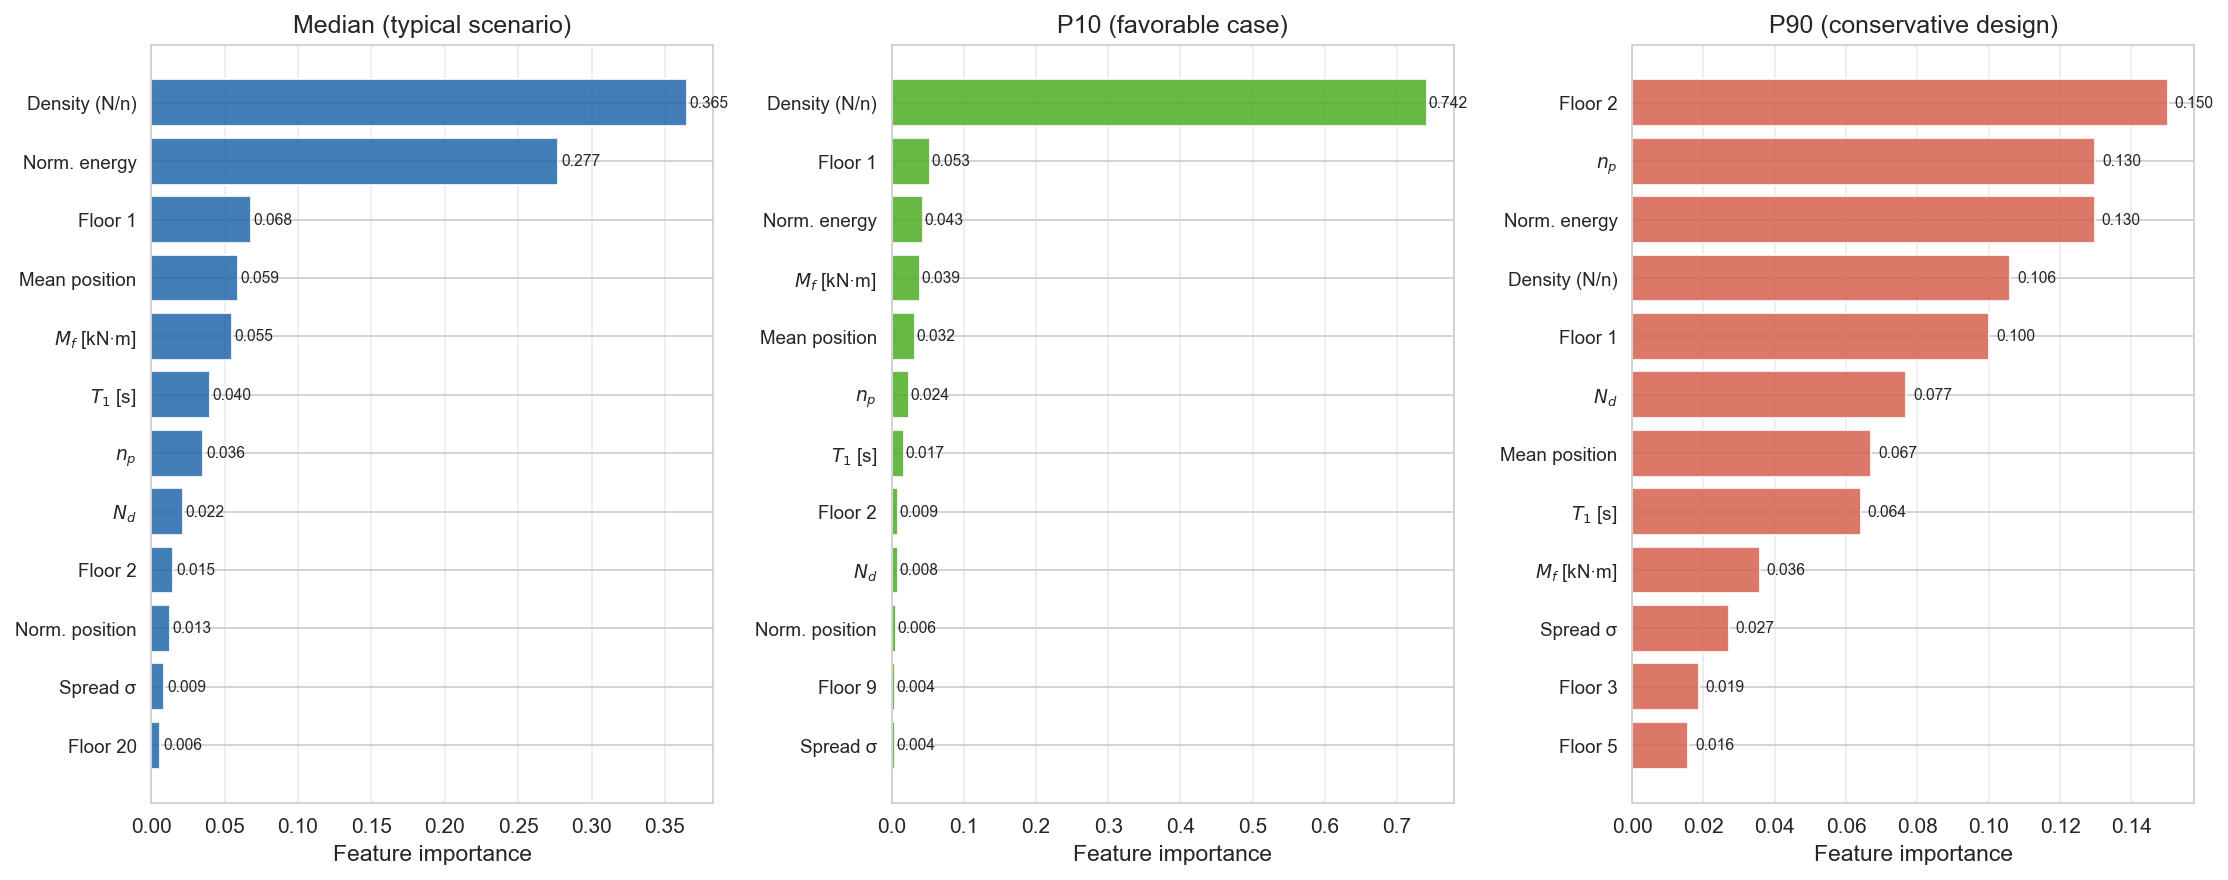
\includegraphics[width=\linewidth]{figs/F4_feature_importance_3targets.png}
\caption{Importancia de características (XGBoost) para los 12 predictores
principales en los tres escenarios de $CR_2$. Los ejes horizontales son
independientes; comparar por orden de importancia, no por magnitud.}
\label{fig:importancia}
\end{figure}

\subsection{Rendimiento Decreciente: Efecto de la Densidad de Amortiguadores}
\label{sec:results:decreciente}

La \cref{fig:decreciente} muestra la relación entre $\etad$ y el mejor $\CR{med}$
alcanzable, estratificada por altura. La mejora es mayor en
$\etad \in [0{,}30,\,0{,}60]$ y se reduce después. El análisis del umbral del
80\,\% (\cref{fig:curvas_internas}) indica que marcos de 6--20 pisos lo alcanzan
con $\etad \approx 0{,}85$. Los marcos de 3--5 pisos necesitan
$\etad \approx 0{,}95$ porque cada dispositivo adicional tiene mayor impacto
proporcional.

Para verificar que esta dominancia de $\etad$ es independiente de las otras
variables, se realizó un análisis de dominancia estocástica en los ocho registros.
Se comparó el percentil~5 de $CR_2$ en un intervalo de densidad alto contra el
percentil~95 del inmediatamente inferior. La dominancia se confirma en los ocho
registros: incluso una configuración desfavorable en $\Mf$ o posición, pero con
mayor densidad, supera al 95\,\% de las de menor densidad. La correlación varía
de $r=-0{,}74$ (El~Centro~1940) a $r=-0{,}55$ (Kobe~1995). La excepción es
Trinidad~1983 ($r=-0{,}18$), cuyas características espectrales de baja
intensidad relativa reducen la demanda de deriva entre pisos, disminuyendo
la influencia de la cobertura global y haciendo que la posición y capacidad
por dispositivo recuperen relevancia.

\begin{figure}[htbp]
\centering
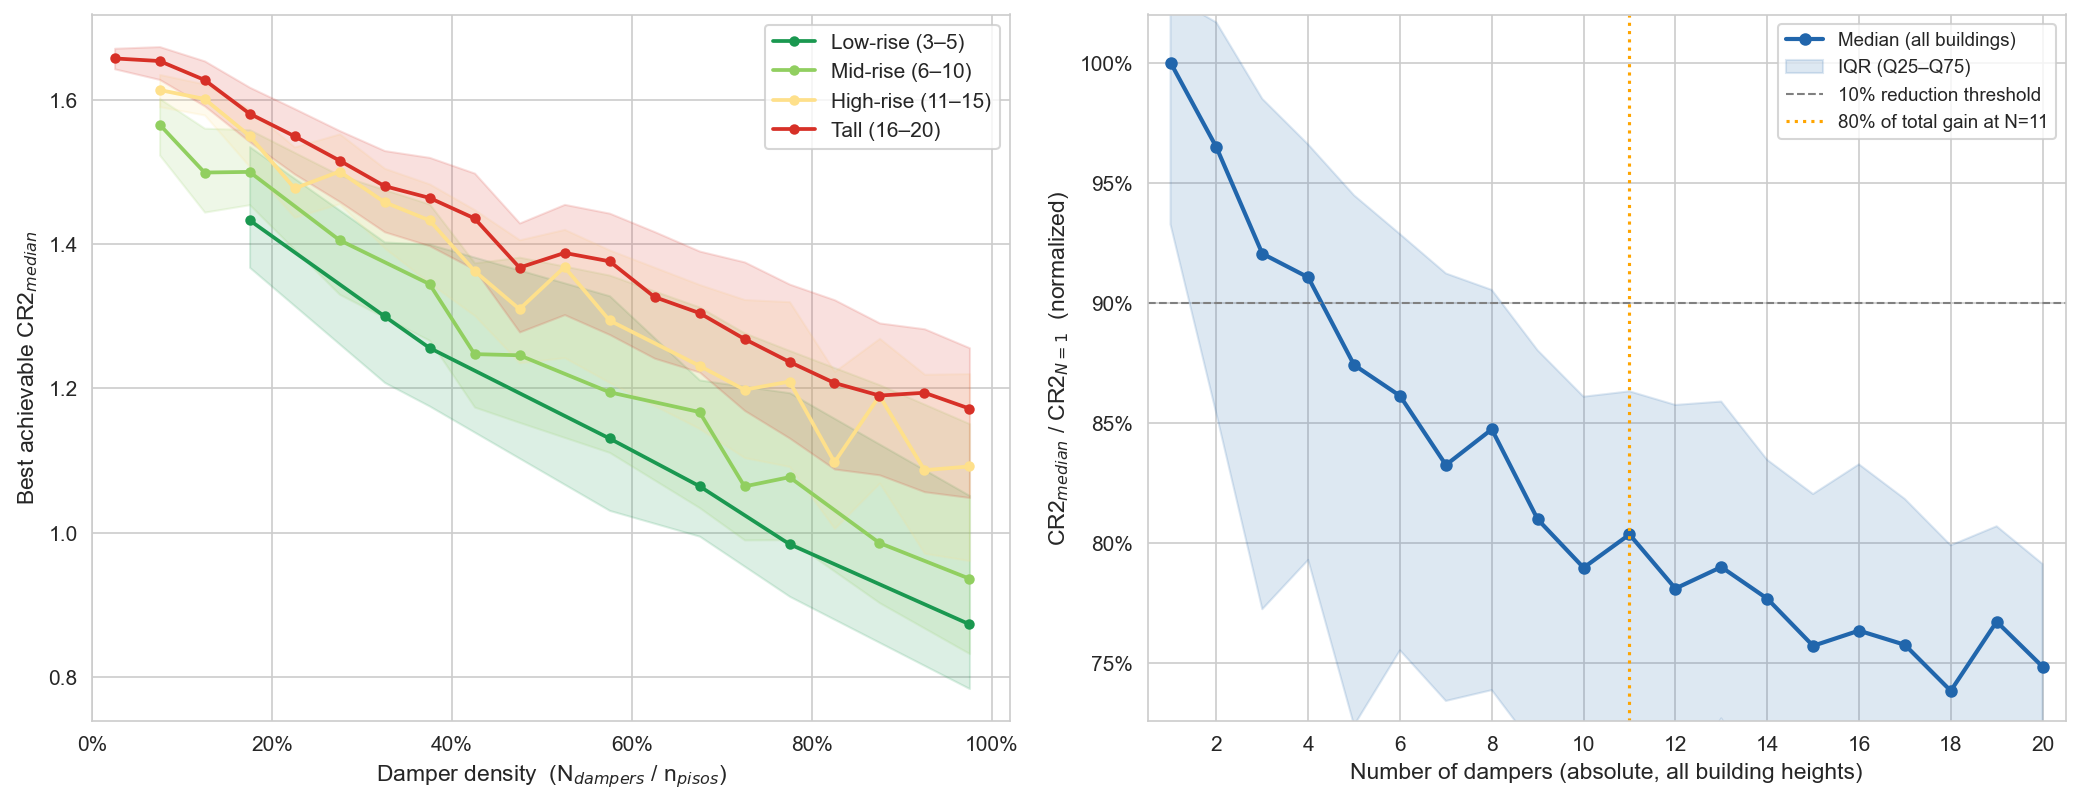
\includegraphics[width=\linewidth]{figs/F5_diminishing_returns.png}
\caption{Izquierda: mejor $\CR{med}$ vs.\ densidad $\etad$, estratificado por
altura (mediana $\pm$ IQR). Derecha: $CR_2$ vs.\ $\nd$ absoluto (confundido
con altura; el panel izquierdo es la comparación apropiada).}
\label{fig:decreciente}
\end{figure}

\begin{figure}[htbp]
\centering
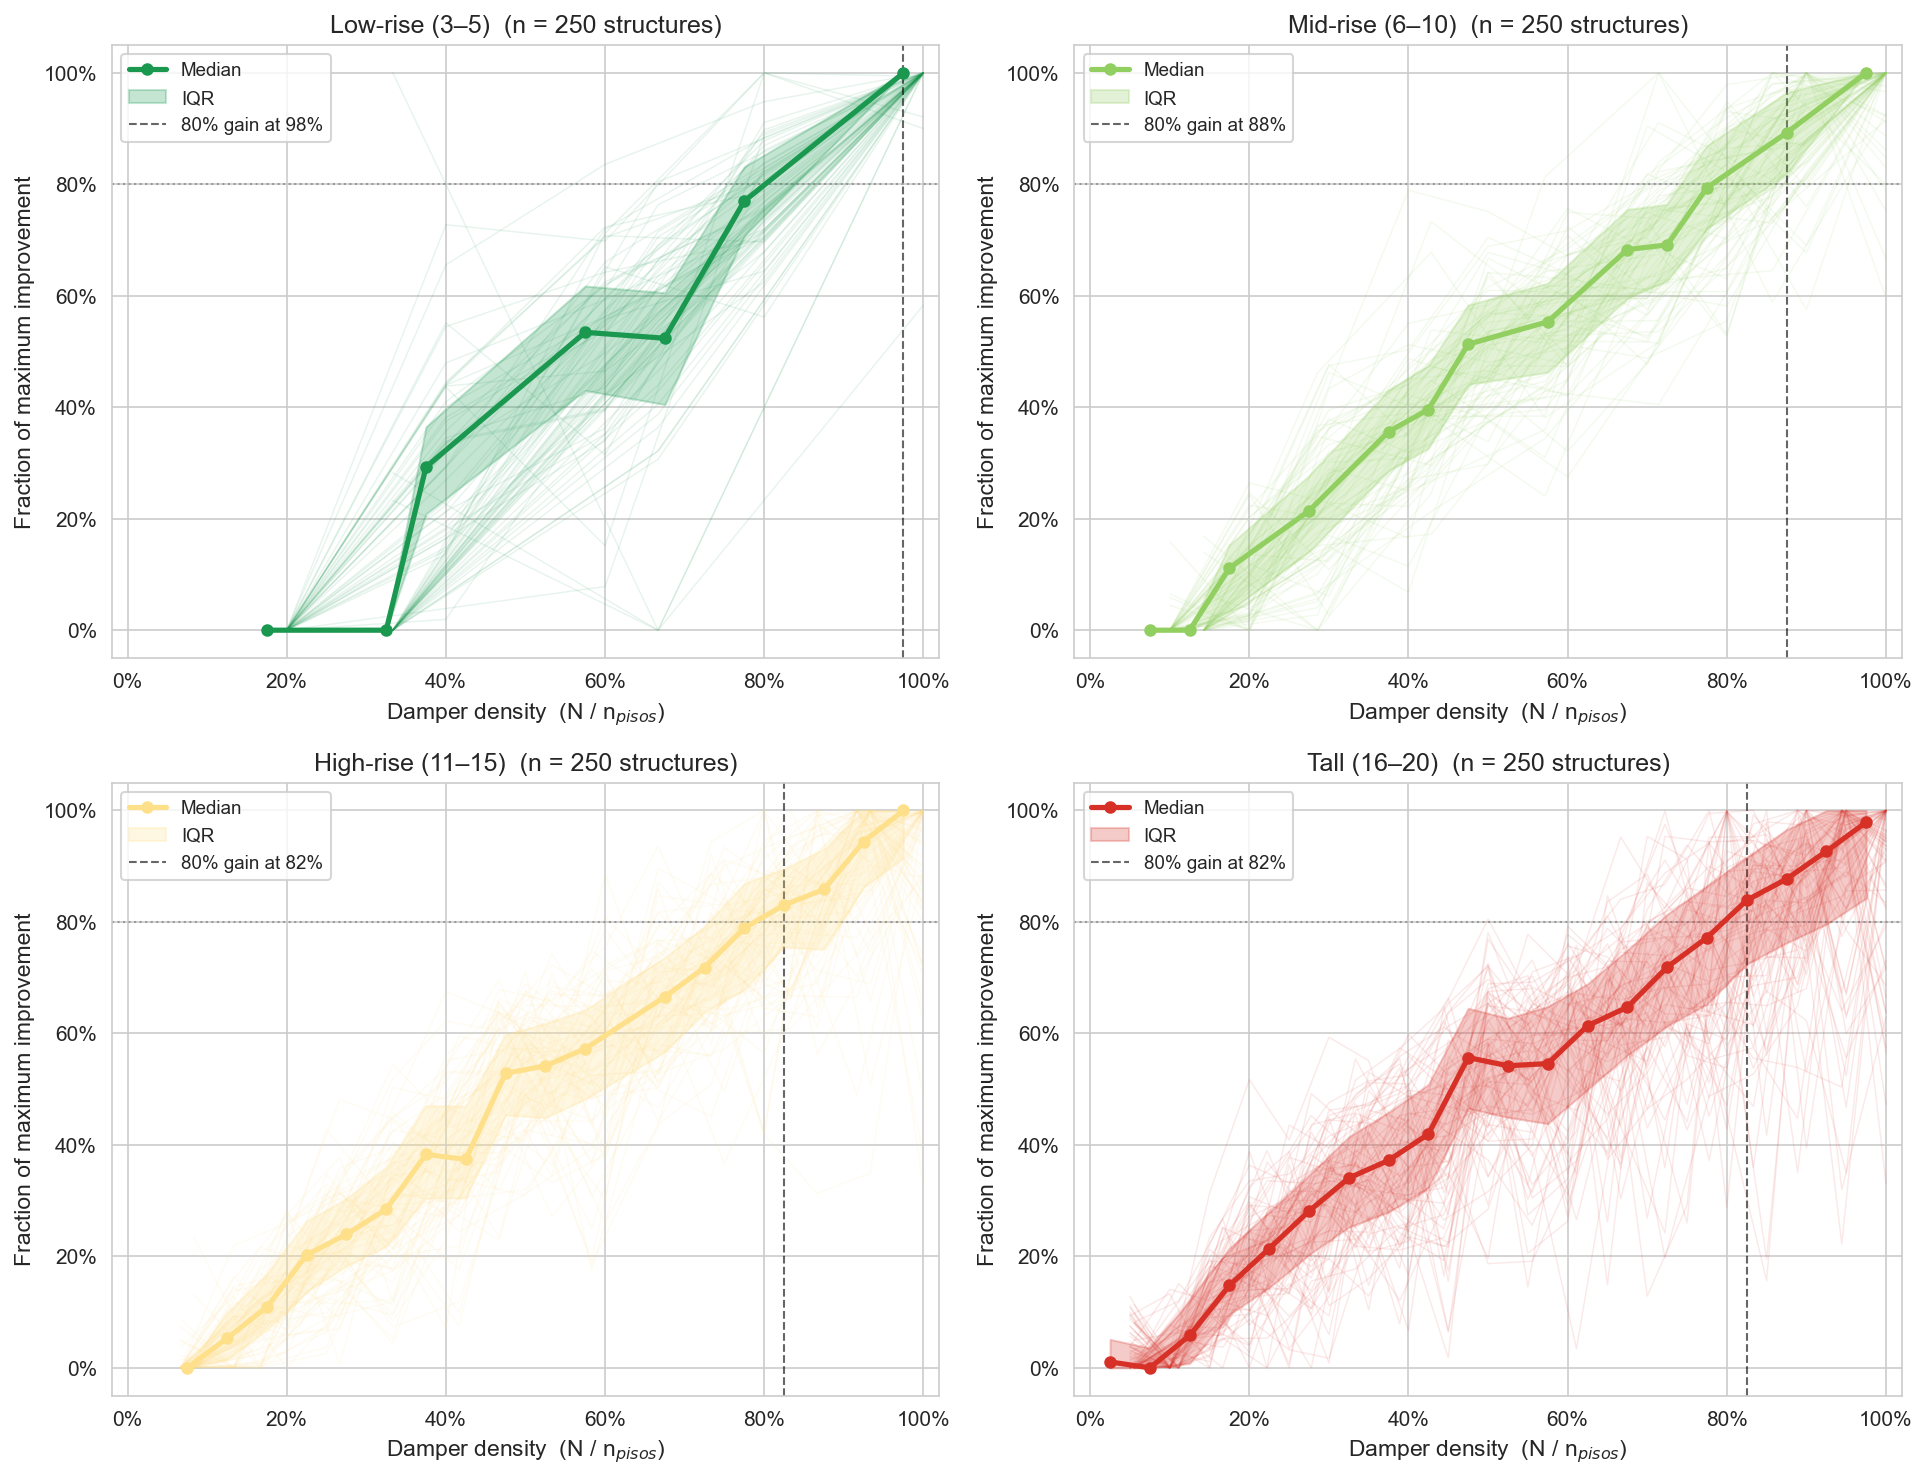
\includegraphics[width=\linewidth]{figs/F6_within_structure_curves.png}
\caption{Curvas de rendimiento decreciente intra-estructura. Cada línea delgada
es una estructura; la gruesa es la mediana $\pm$ IQR. Línea punteada: densidad
donde se alcanza el 80\,\% de la ganancia máxima.}
\label{fig:curvas_internas}
\end{figure}

\subsection{Interacción entre Cantidad de Amortiguadores y Momento Friccional}
\label{sec:results:interaccion}

La \cref{fig:mapa_calor} muestra el $CR_2$ mediano en función de $\nd$ y $\Mf$
binados, estratificado por: bajo (3--5 pisos), medio (6--12 pisos) y alto
(13--20 pisos).

En los tres grupos, baja densidad con $\Mf \leq 100$\KM produce el peor
desempeño. En marcos bajos, $\nd$ y $\Mf$ contribuyen por igual: subir $\nd$ de
1--2 a 3--4 reduce $CR_2$ de 1{,}46 a 1{,}12, y subir $\Mf$ de 100 a 300\KM
produce mejoras similares. En marcos medios y altos, $\nd$ domina: subir $\Mf$
sigue ayudando ($\Delta CR_2 \approx 0{,}37$--$0{,}46$), pero agregar
dispositivos tiene mayor efecto. En ningún grupo se observa insensibilidad a
$\Mf$: incluso con $\nd \geq 11$, la diferencia entre $\Mf < 100$\KM y
$\Mf > 400$\KM es de 0{,}46 unidades en marcos medios.

Las configuraciones óptimas se concentran en $\Mf \in [300,\,460]$\KM
(mediana 400\KM, IQR [269,\,456]\KM) con coberturas cercanas a la unidad.

\begin{figure}[htbp]
\centering
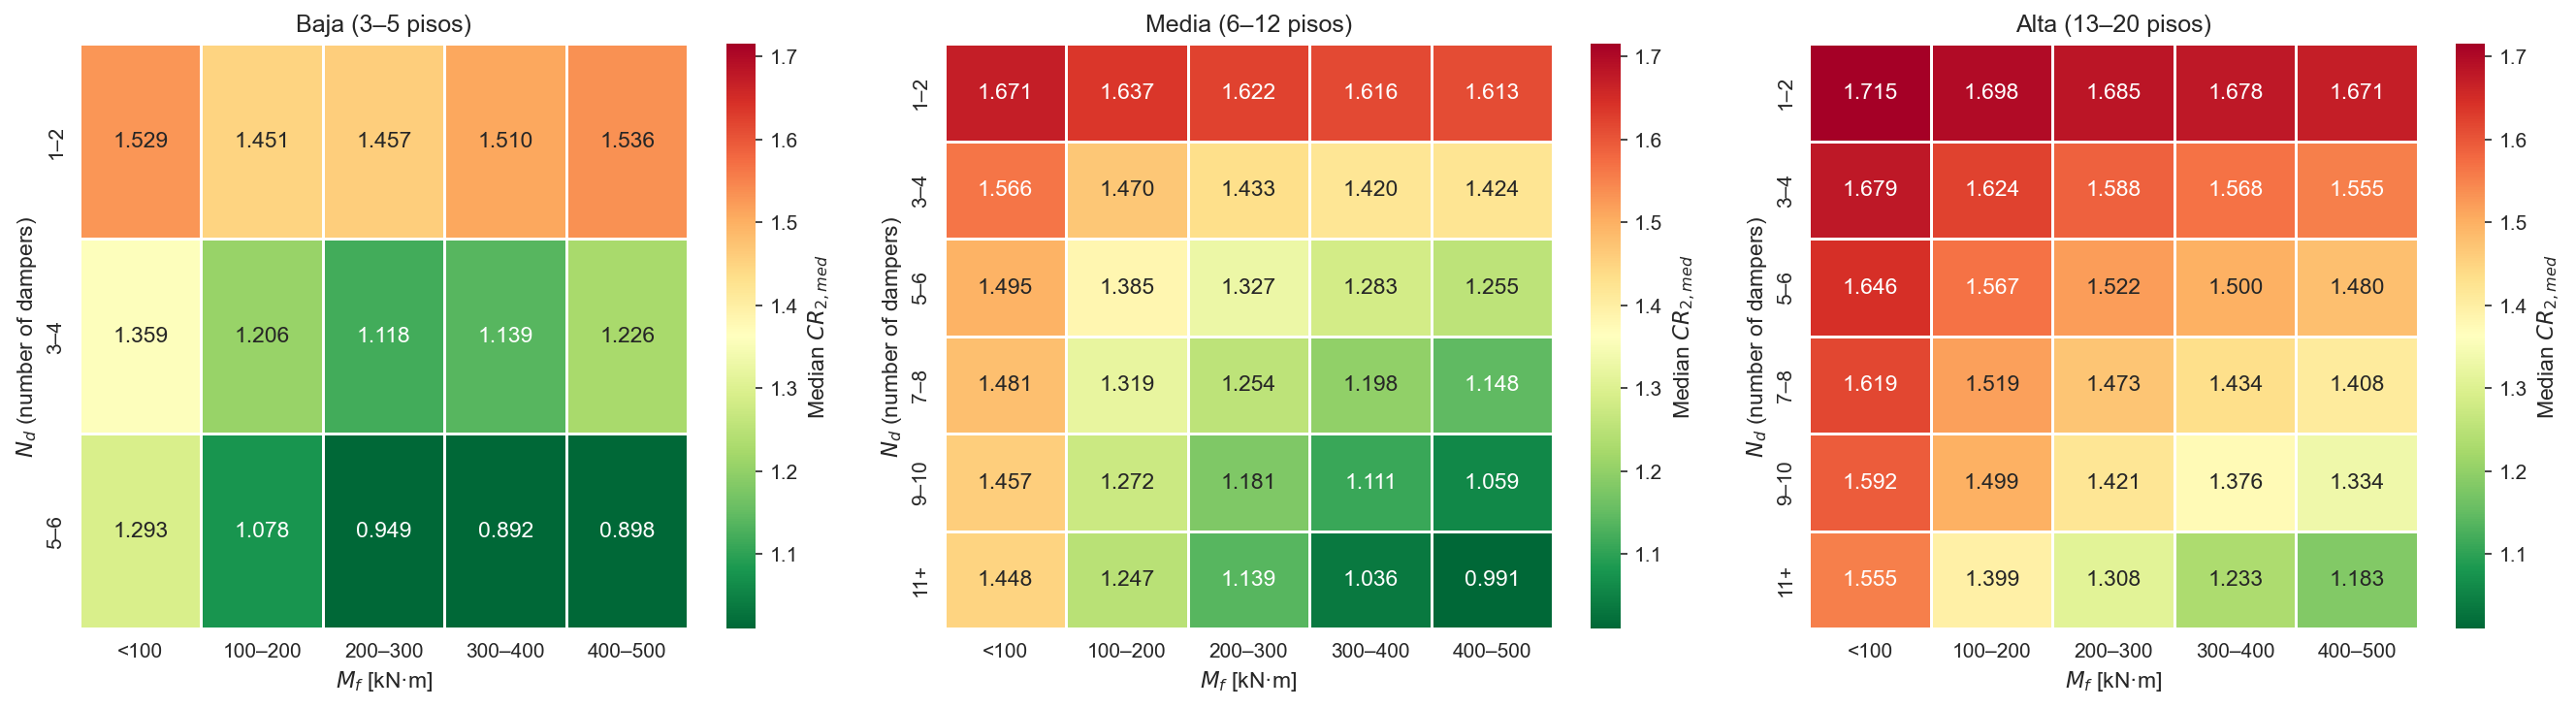
\includegraphics[width=\linewidth]{figs/F7_interaction_heatmap.png}
\caption{$CR_2$ mediano en función de bins de $\nd$ y $\Mf$ (kN$\cdot$m),
estratificado por altura: bajo (3--5), medio (6--12) y alto (13--20 pisos).
Escala de color consistente entre paneles.}
\label{fig:mapa_calor}
\end{figure}

\subsection{Convergencia del Diseño entre Escenarios Sísmicos}
\label{sec:results:convergencia}

La \cref{fig:convergencia} muestra que el $\nd$ recomendado es consistente entre
escenarios: mediana y P10 producen recomendaciones casi idénticas. P90 tiende a
pedir un $\nd$ mayor en edificios altos, pero la diferencia es menor de 2 en el
80\,\% de los casos. Un diseño para la mediana protege casi óptimamente frente
a toda la variabilidad del ensemble.

\begin{figure}[htbp]
\centering
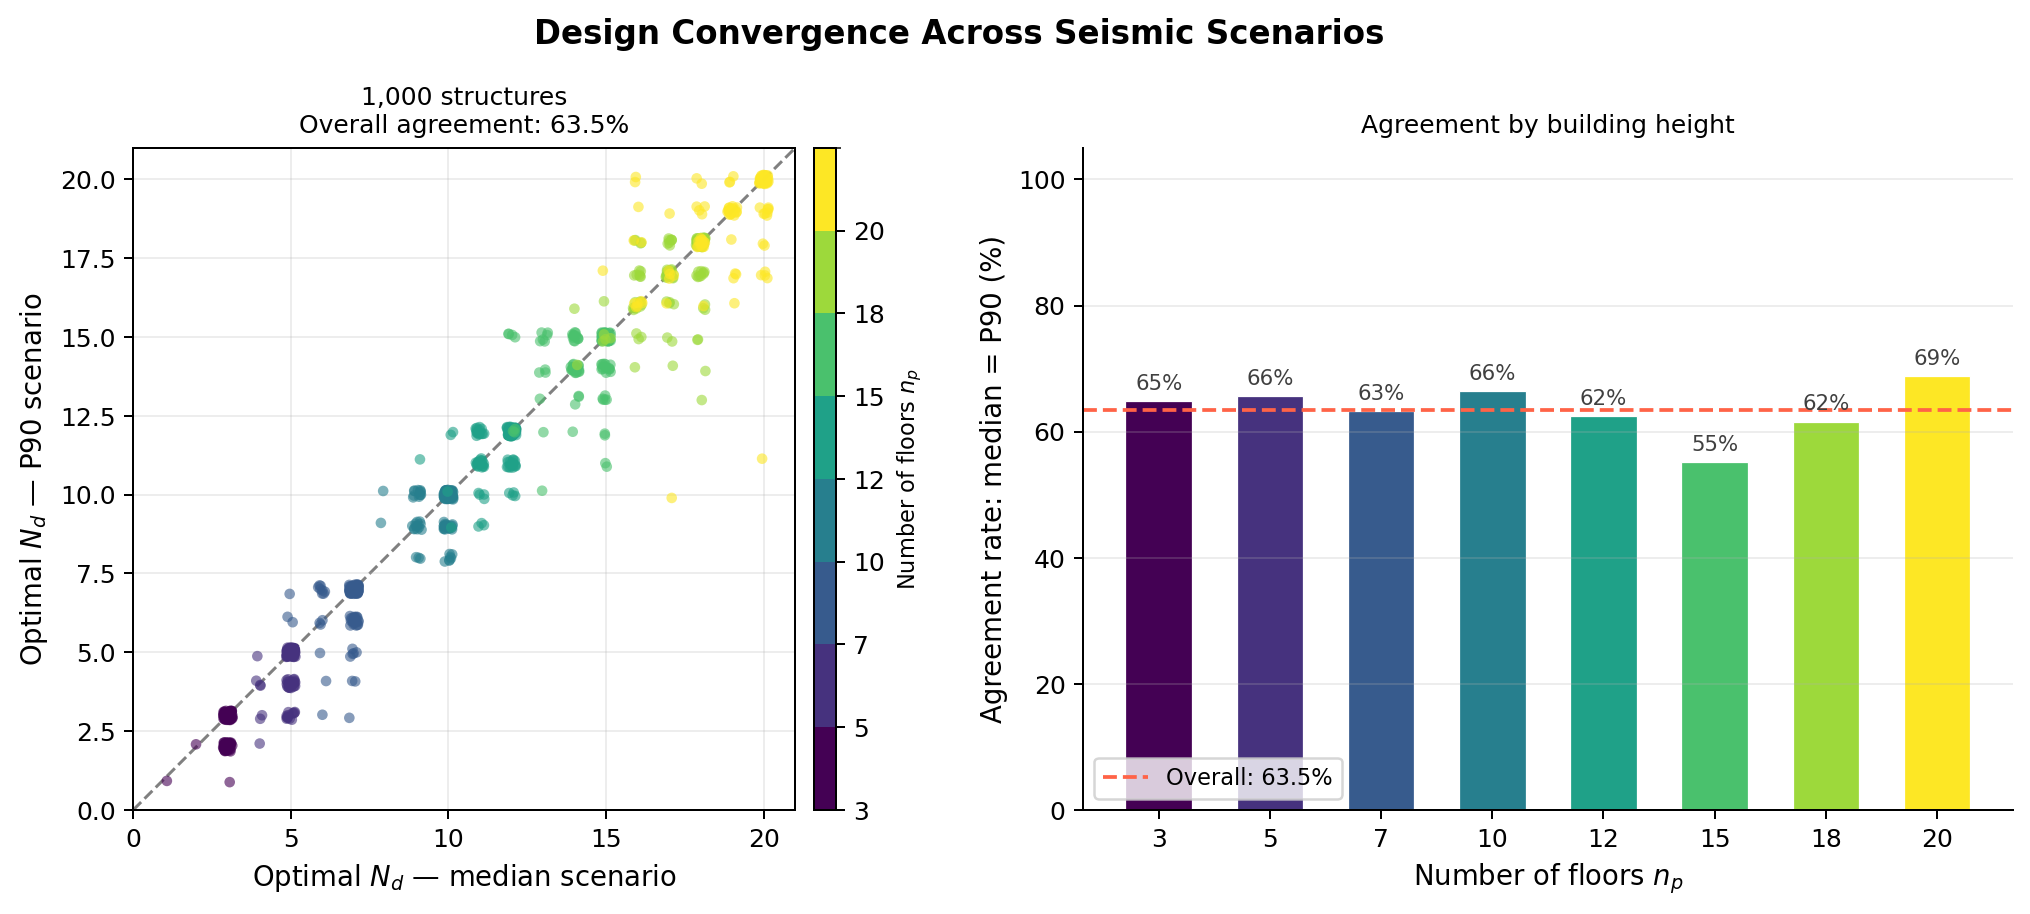
\includegraphics[width=\linewidth]{figs/F8_convergence_extended.png}
\caption{Izquierda: $\nd$ recomendado por escenario en 1\,000 estructuras.
Derecha: acuerdo y discrepancia $|\nd^{\mathrm{P90}} - \nd^{\mathrm{med}}|$
por altura $\np$.}
\label{fig:convergencia}
\end{figure}

%%═══════════════════════════════════════════════════════════════════════════
\section{Discusión}
\label{sec:discussion}
%%═══════════════════════════════════════════════════════════════════════════

\subsection{La Densidad de Cobertura como Variable Dominante}

La densidad $\etad = \nd/\np$ emerge como el predictor más influyente de $CR_2$
($r = -0{,}73$) y su dominancia es robusta frente a los ocho registros sísmicos
(\cref{sec:results:decreciente}). Con base en el análisis del umbral del 80\,\%
de ganancia máxima, se derivan las siguientes recomendaciones de diseño:
$\etad \geq 0{,}85$ para marcos de mediana y gran altura (6--20~pisos), y
$\etad \geq 0{,}95$ para marcos de baja altura (3--5~pisos).

\subsection{Reconciliación con Jarrahi et al.\ (2020): Criterio Energético vs.\ Criterio de Desplazamiento}

\citet{Jarrahi2020sdee} reportaron que la función objetivo energética
$f = E_i / E_{\mathrm{AFR}}$ se satura en $\etad \approx 0{,}60$ para un
MARM de 10~pisos, lo cual coincide con el punto en que la energía histéretica
acumulada $E_h$ del marco estructural cae a cero (la estructura deja de
plastificar). El presente estudio, utilizando $CR_2$, encuentra la saturación
en $\etad \approx 0{,}85$ para la misma categoría de altura. La diferencia
refleja la sensibilidad de la métrica: el criterio energético detecta el inicio
de un estado elástico estructural como un umbral binario; $CR_2$ continúa
diferenciando configuraciones una vez suprimida la plastificación, capturando
la amplificación residual del desplazamiento y las demandas de aceleración.
Los dos umbrales son por tanto complementarios:
\begin{itemize}
    \item $\etad \geq 0{,}60$: prevención de daño estructural (criterio de
          \citealt{Jarrahi2020sdee}, basado en energía);
    \item $\etad \geq 0{,}85$: control de serviciabilidad ---la aceleración
          absoluta máxima ($R_2$, ec.~\ref{eq:R_individual}) y el cortante
          basal ($R_3$) dejan de responder significativamente a una cobertura
          adicional, reduciendo la demanda sobre componentes no estructurales
          y sistemas de instalaciones.
\end{itemize}
Un diseño orientado únicamente a la protección estructural debe satisfacer el
primer criterio; uno que adicionalmente controle la respuesta de aceleración
---gobernante para componentes no estructurales sensibles a la inercia---
debe apuntar al segundo, tal como está implícito en la formulación de $CR_2$
(ec.~\ref{eq:CR}), que integra simultáneamente $R_1$, $R_2$ y $R_3$.

\subsection{Interacción entre Momento Friccional y Cobertura}

El análisis del mapa de calor (\cref{fig:mapa_calor}) revela una relación de
sustitución entre $\nd$ y $\Mf$ a niveles de cobertura intermedios: duplicar
$\Mf$ con un conteo fijo produce reducciones de $CR_2$ similares a incrementar
$\nd$ en dos pisos. Esta interacción no queda capturada por el análisis de
correlación marginal y motiva el uso de modelos ML de ensemble que representan
explícitamente las interacciones no lineales entre características. El rango óptimo identificado por ML, $\Mf \in [300,\,460]$\KM, es consistente
con los valores reportados en la Tabla~3 de \citet{Jarrahi2020sdee} para el
caso de 6~amortiguadores en un MARM de 10~pisos (81--439\KM), y con el rango
350--450\KM identificado por \citet{Ponce2026} para el mismo tipo de
estructura bajo un enfoque probabilístico.

\subsection{Robustez entre Escenarios}

El alto nivel de acuerdo entre las recomendaciones de diseño de los escenarios
de mediana y P90 (\cref{fig:convergencia}) implica que no es necesario resolver
problemas de optimización separados para diferentes niveles de peligro sísmico
cuando el objetivo es identificar el $\nd$ óptimo. El enfoque multi-registro
aborda directamente la limitación de los estudios de optimización con un único
registro \citep{Jarrahi2020jbe,Jarrahi2020sdee}, capturando la variabilidad
registro-a-registro en las estadísticas P10, mediana y P90, lo que hace a las
recomendaciones ML inherentemente robustas frente a la incertidumbre en la
selección de acelerogramas.

\subsection{Limitaciones}

Se deben reconocer las siguientes limitaciones. (i)~Los modelos estructurales son marcos cortantes elásticos idealizados; la
interacción no lineal marco--AFR no queda capturada explícitamente. Los
resultados son por tanto aplicables a niveles de demanda sísmica en que la
respuesta del marco permanece elástica o cuasielástica; para sismos de alta
intensidad con plastificación significativa del marco se esperan desviaciones
respecto a las recomendaciones aquí derivadas. (ii)~Los ocho acelerogramas, aunque sísmicamente
diversos, pueden no representar todos los entornos tectónicos relevantes.
(iii)~La validación del modelo se basa únicamente en validación cruzada; un
conjunto de prueba independiente proporcionaría una evaluación de generalización
más rigurosa. (iv)~Se asume un valor uniforme de $\Mf$ por estructura; las
distribuciones de $\Mf$ específicas por piso pueden ser preferibles en la
práctica. (v)~No se incorpora ninguna función de costo, por lo que la
optimización económica de la fracción de cobertura no se aborda.

%%═══════════════════════════════════════════════════════════════════════════
\section{Conclusiones}
\label{sec:conclusions}
%%═══════════════════════════════════════════════════════════════════════════

Las siguientes conclusiones principales se derivan del análisis de
$\approx$434\,000 simulaciones tiempo-historia no lineales sobre 1\,000
configuraciones estructurales diversas y ocho registros sísmicos reales:

\begin{enumerate}

\item \textbf{Precisión del modelo sustituto ML.}
XGBoost y Random Forest alcanzaron $\Rsq$ de 0{,}92--0{,}93 para $\CR{med}$ y
$\CR{P10}$, y 0{,}84 para $\CR{P90}$. Los modelos de ensemble redujeron el error
de predicción en $\approx$49\,\% respecto a los baselines lineales, cuantificando
la estructura no lineal de la relación diseño--desempeño.

\item \textbf{Umbral de rendimiento decreciente: $\etad \approx 0{,}85$.}
El análisis intra-estructura revela que el 80\,\% de la reducción máxima de
$CR_2$ se alcanza con $\etad \approx 0{,}85$ para marcos de mediana y gran
altura (6--20~pisos) y con $\etad \approx 0{,}95$ para marcos de baja altura
(3--5~pisos). Estos umbrales proveen criterios prácticos de costo-efectividad
para el despliegue de AFR. Complementariamente, el $\Mf$ óptimo identificado
por el modelo ML se concentra en [300,\,460]\KM (mediana 400\KM); para
$\etad \geq 0{,}75$, $CR_2$ es relativamente insensible al valor específico
de $\Mf$ dentro de [200,\,500]\KM, por lo que la fracción de cobertura es
el parámetro de diseño más determinante.

\item \textbf{Reconciliación con el umbral energético de Jarrahi et al.}
\citet{Jarrahi2020sdee} reportaron la saturación del objetivo energético en
$\etad \approx 0{,}60$ (plastificación estructural eliminada). El presente
criterio basado en desplazamiento encuentra la saturación en $\etad \approx
0{,}85$, 25 puntos porcentuales más alto. La diferencia se explica por la mayor
sensibilidad de $CR_2$ a las demandas de desplazamiento y aceleración que
persisten más allá del umbral de plastificación. Los dos criterios describen
niveles de desempeño complementarios: $\etad \geq 0{,}60$ apunta a la
prevención de daño estructural; $\etad \geq 0{,}85$ adicionalmente controla
la serviciabilidad.

\item \textbf{Robustez entre escenarios.}
El $\nd$ óptimo recomendado por los escenarios de mediana y P90 difiere en menos
de 2~pisos en el 80\,\% de las estructuras analizadas, confirmando que un diseño
optimizado para la mediana proporciona protección casi óptima frente a toda la
variabilidad sísmica del ensemble de ocho registros.

\item \textbf{Trabajo futuro.}
Las extensiones deben incorporar comportamiento inelástico del marco,
distribuciones de $\Mf$ específicas por piso, restricciones de costo de
instalación y suites de registros sísmicos más amplias que representen diferentes
entornos tectónicos. La validación experimental para configuraciones multi-piso
y la integración de los modelos entrenados en una herramienta de diseño
interactiva constituyen direcciones inmediatas de investigación.

\end{enumerate}

%%═══════════════════════════════════════════════════════════════════════════
\section*{CRediT Author Contribution Statement}

\textbf{E.~Ponce}: Conceptualization, Methodology, Software, Formal Analysis,
Investigation, Validation, Data Curation, Visualization, Writing -- Original Draft.
\textbf{H.~Yañez-Godoy}: Conceptualization, Supervision, Writing -- Review \& Editing.

\section*{Declaration of Competing Interests}

The authors declare that they have no known competing financial interests or
personal relationships that could have appeared to influence the work reported
in this paper.

\section*{Funding}

This research did not receive any specific grant from funding agencies in the
public, commercial, or not-for-profit sectors.

\section*{Acknowledgements}

The first author gratefully acknowledges the financial support provided by the
Secretaría de Ciencias, Humanidades, Tecnología e Innovación (SECIHTI, Mexico)
through a master's scholarship. The authors also acknowledge the institutional
support of the Universidad Autónoma de Querétaro (UAQ, Mexico) and the Institut
de Mécanique et d'Ingénierie (I2M, UMR CNRS 5295), University of Bordeaux,
France.

\section*{Declaration of Generative AI and AI-Assisted Technologies in the
Writing Process}

During the preparation of this work the authors used Claude (Anthropic) in order
to assist with translation from Spanish to English and language style correction.
After using this tool, the authors reviewed and edited the content as needed and
take full responsibility for the content of the publication.

%%═══════════════════════════════════════════════════════════════════════════
\bibliographystyle{elsarticle-harv}
\bibliography{references}

\end{document}
